\documentclass[12pt]{article}

\usepackage{listings}
\lstset{
  language=Python
}

\usepackage{graphicx}
\graphicspath{ {../resources/green-sky/} }

\usepackage[margin=1in]{geometry}

\usepackage[colorlinks]{hyperref}
\hypersetup{
  urlcolor = {cyan}
}

\title{Why Doesn't The Sky Turn Green?}
\author{Rushi Shah}
\date{09 November 2015}

\begin{document}

  \maketitle

I was leafing through the US Army Corps of Engineers'
\href{\%7B\%7B\%20site.url\%20\%7D\%7Dblog/resources/Remote-Sensing-Army-Manual.pdf}{Manual
on Remote Sensing} and learned about how Rayleigh scattering creates
blue skies during the day and redish-orange sunsets. Well, everybody
knows about blue skies and red sunsets, was the title just click-bait,
you ask? No, but I'll get to that.

\section{The Basics of Rayleigh
Scattering}\label{the-basics-of-rayleigh-scattering}

Let's start with this whole Rayleigh scattering thing. Basically the
idea is that particles in the atmosphere (like Oxygen and Nitrogen
particles) scatter rays of light as they enter the atmosphere.

How much the light is scattered is heavily dependent on the wavelength
of the light. Remember how ROY-G-BIV represents the colors of the
rainbow (and thus the spectrum of visible light)? Well that spectrum of
light starts with long wavelength rays (reds, oranges, and yellows) and
ends with short wavelength rays (blues, indigos, and violets).

\begin{center}
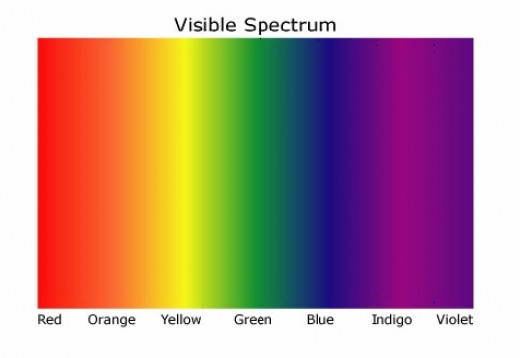
\includegraphics[width=5in]{spectrum}
\end{center}

The amount of light that is scattered (denoted with the variable I) is
highly inversely proportional to the wavelength of the light (denoted
with the greek letter λ). Put simply, as the wavelength goes down, the
light waves are scattered more quickly.

\begin{displaymath}
  I \propto \frac{1}{\lambda^4}
\end{displaymath}

When sunlight hits the earth directly during mid-day, it travels through
a small amount of atmosphere, and thus we see the wavelengths of light
that are immediately scattered. Based on the equation above, the blues,
indigos, and violets would be scattered first (and they blend together
into the blue sky we see).

% \begin{figure}[htbp]
% \centering
% \includegraphics{http://www.givingwhatwecan.org/sites/givingwhatwecan.org/files/Krisztina\%20Csortea/Create\%20Story/blue_sky.jpg}
% \caption{Blue sky}
% \end{figure}

As the sun sets, it goes through more and more particles to reach us.
The short wavelength rays have already been scattered, and by the time
the light reaches us, the particles can only scatter the light
remaining. Thus the reds, oranges, and yellows are scattered near us and
the sunset seems red-ish or orange-ish.

% \begin{figure}[htbp]
% \centering
% \includegraphics{http://www.effifoods.com/blog/wp-content/uploads/2015/05/red-orange-sunset.jpg}
% \caption{Red orange sunset}
% \end{figure}


\section{\texorpdfstring{What about the Green,
\href{http://www.shmoop.com/great-gatsby/green-light-symbol.html}{Old
Chap}?}{What about the Green, Old Chap?}}\label{what-about-the-green-old-chap}

Well, one might be satisfied with that explanation and inclined to stop
there, but wasn't the spectrum ROY\textbf{G}BIV? Why is the sky never
green as the sun begins to set?

There are a few possible explanations.

The first would be that the green is simply washed out by the more
powerful colors like blue and orange, and that we simply don't percieve
the green. This would be supported by the fact that our perception is
heavily influenced by our eyes, and the fact that
\href{http://physics.stackexchange.com/a/28903}{we see more blue in the
day-time sky than indigo or violet}. If that was the case, maybe if you
looked hard enough you might see it, such as the subtle green boundary
in this image:

\begin{center}
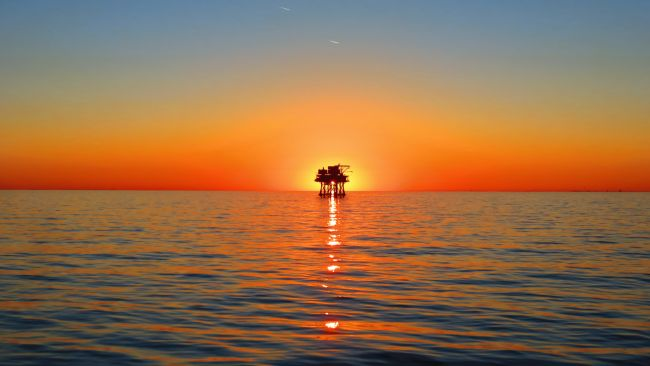
\includegraphics[width=6in]{green-sky.jpg}
\end{center}

The second might be the
\href{https://www.youtube.com/watch?v=gGgcZkxEWEc}{legendary green
flash}. However, it seems that the whole green flash business is more of
a mirage than a representation of the green wavelengths.
\href{http://physics.stackexchange.com/a/137211}{This Physics Stack
Exchange answer} outlines what the green flash really is. Furthermore,
the green flash is rumored to appear just as the sun dips below the
horizon, which is not where the spectrum implies it should be. Any green
light as a result of the Rayleigh scattering should manifest itself
directly after the blue scattering and directly before the red
scattering, not after the red scattering.

The third, most physics/mathematically based explanation is that the
window of opportunity for us to see green is so miniscule that it would
be unrealistic for us to percieve it. As stated in
\href{http://hyperphysics.phy-astr.gsu.edu/hbase/atmos/redsun.html}{this
hyper-physics explanation}:

\begin{quote}
The index of refraction of air for red is 1.000292 and that for blue is
1.000295. Out of a total refraction of about 0.53°, the dispersion is
only 0.006° or about 20 arc seconds, compared to a 120 arc sec
resolution for the eye. Thus under normal conditions the eye would not
see the separation of red and blue images of the sun.
\end{quote}

This small index of refraction difference implies that the shift from
blue to red is almost imperceptible, and has no space for us to
recognize the green in the sky.

\section{Further reading:}\label{further-reading}

\begin{itemize}
\item
  \href{http://physics.stackexchange.com/a/137217}{Physics Stack
  Exchange on why the sky is never green}
\item
  \href{http://physics.stackexchange.com/a/28903}{Physics Stack Exchange
  on why the sky is not purple}
\item
  The Rayleigh Scattering section on page 2-15 in the
  \href{\%7B\%7B\%20site.url\%20\%7D\%7Dblog/resources/Remote-Sensing-Army-Manual.pdf}{US
  Army Corps of Engineers Manual on Remote Sensing}
\item
  \href{http://hyperphysics.phy-astr.gsu.edu/hbase/atmos/redsun.html}{Hyper-Physics
  explanation of the green flash}
\item
  \href{http://news.nationalgeographic.com/news/2013/10/131027-sunset-sky-change-color-red-clouds-science/}{A
  simple explanation of the red sunsets and blue sky phenomenon from
  National Geographic}
\end{itemize}

\end{document}
